\documentclass[UTF8]{article}
\usepackage[margin=1in]{geometry} % 设置边距,符合Word设定
\usepackage{lipsum}
\usepackage{float}
\usepackage{amsmath}
\usepackage{tabularx}
\usepackage{graphicx}
\usepackage{amsfonts} 


\title{The oleic acid induction system model (latex version)}
\author{LZU-CHINA}
\date{\today}
\begin{document}
    \maketitle
    \begin{abstract}

    \end{abstract}

\section{Mechanism}

From the oleic acid induction mechanism, we can divide the expression of the FadR promoter into the following two scenarios, as shown in Figure \ref{fig:Mechanism}:
\begin{itemize}
	\item With oleic acid: $\rightarrow$ acyl-CoA A $\rightarrow$ FadR protein departs from promoter PfadB $\rightarrow$ gene expresses normally, $\beta$-oxidation initiates.
	\item Without oleic acid: $\rightarrow$ FadR protein binds to promoter PfadB $\rightarrow$ gene expression is inhibited.
\end{itemize}

\begin{figure}[h]
	\centering
	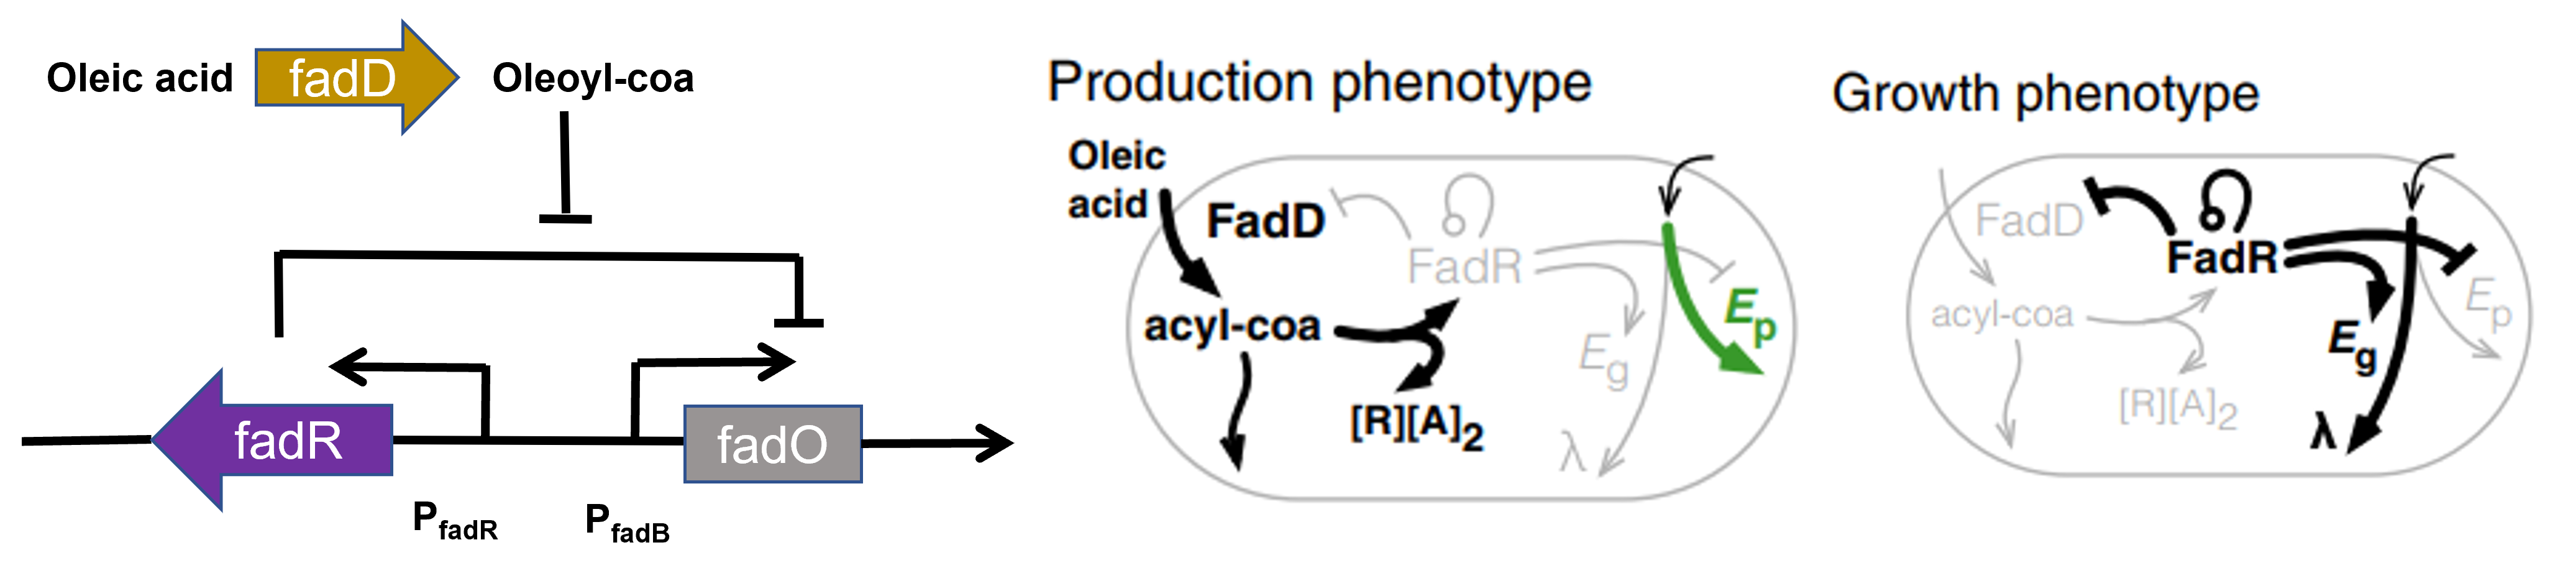
\includegraphics[width=0.8\linewidth]{figures/mech.png}
	\caption{Model Mechanism}
	\label{fig:Mechanism}
\end{figure}
The balance of oleic acid synthesis metabolism and decomposition metabolism in microorganisms is controlled by the transcriptional regulatory factor FadR. In the absence of oleic acid, it's a Growth phenotype with native negative autoregulation (NAR) . At this time, fatty acid synthesis metabolism is activated. FadR binds to the promoter p-fadB of the bacterial $\beta$-oxidation pathway gene fadO, inhibiting the expression of fadO, thereby inhibiting bacterial $\beta$-oxidation. In the presence of excess oleic acid, it's a Production phenotype with engineered positive autoregulation (PAR) . Fatty acid degradation metabolism is activated. After FadR couples with oleic acid, it departs from the promoter p-fadB of fadO, allowing fadO expression, and bacterial $\beta$-oxidation is completed.


\section{Model Assumptions}

\begin{enumerate}
	\item The activation state of the oleic acid inducer (corresponding to the presence/absence of oleic acid environment) can be determined by the concentration of the regulator FadR. The expression of the product synthesis enzyme and the synthesis of the product itself depend on the control factor FadR. Therefore, we only define the state of the oleic acid inducer by the concentration of FadR.
	\item FadD expression is solely controlled by FadR. In native E. coli, the  expression of FadD under aerobic conditions is co-regulated by FadR and  the CRP-cAMP complex (EcoCyc). However, in the presence of common carbon sources like glucose, the expression level of CRP-cAMP is very low, so  its effect can be neglected.
	\item The expression rate of the enzyme in two oleic acid inducer states can be modeled in the form of a Hill function. Studies have shown that the expression of gene products takes the form of a Hill function [4], either as $P_T(T)=\frac{a \cdot(K \cdot T)^n}{1+(K \cdot T)^n}$ for $T$-activated expression, or as $P_T(T)=\frac{a}{1+(K \cdot T)^n}$ for $T$-inhibited expression, where $a$ is the maximum expression rate, $K$ is the affinity with which transcription factor $T$ binds to the operator and controls expression, and $n$ is the Hill coefficient.
	\item The growth rate of engineered bacteria linearly depends on the growth-related enzyme Eg. According to research by Usui et al. [3], the cell growth rate decreases in an approximately linear fashion. We capture this phenomenon and define the growth rate of the cell using a linear function as follows: $\lambda\left(E_g\right)=E_g \cdot \lambda_{\min }+\left(\lambda_{\max }-\lambda_{\min }\right)$. Where $\lambda_{\min }$ and $\lambda_{\max }$ represent the growth rates at zero and maximum expression of $E_g$, respectively.
	\item Enzymes and transcription factors do not undergo active degradation. To  our knowledge, proteins in the system we study are not actively  degraded. Over the duration of cell doubling, protein dilution through  cell growth and division is the main way proteins are lost from the  system, so we model the decay of protein $E$ as growth dilution $\lambda \cdot E$.
\end{enumerate}

\section{Model Establishment}

Our endogenous system model is inspired by the model of Ahmad A. Mannan et al.[1] and the model of Hartline et al.[2], which models the expression rates of the transcription factor FadR, uptake enzyme FadD, and growth-related enzyme $E_g$ [5] using Hill functions as $r_{\mathrm{x}, \mathrm{R}}=P_{\mathrm{R}}(R), r_{\mathrm{x}, \mathrm{D}}=P_{\mathrm{D}}(D)$, $r_{\mathrm{x}, \mathrm{E}_{\mathrm{g}}}=P_{\mathrm{g}}\left(g\right)$. 
\begin{equation}
	\begin{aligned}
		& r_{\mathrm{x}, \mathrm{R}}=b_{\mathrm{R}}+P_{\mathrm{R}}(R), 
		\quad r_{\mathrm{x}, \mathrm{D}}=b_{\mathrm{D}}+P_{\mathrm{D}}(D), 
		\quad r_{\mathrm{x}, E_{\mathrm{g}}}= P_{\mathrm{g}}(g)
	\end{aligned}
\end{equation}

The reaction kinetics of FadD $\left(r_{\mathrm{D}}\right)$ and the reaction kinetics of the acyl-CoA-consuming reaction PIsB $\left(r_{\mathrm{B}}\right)$ are modeled as Michaelis-Menten equations, resulting in:
\begin{equation}
r_{\mathrm{D}}=\frac{k_{\mathrm{cat}, \mathrm{D}} \cdot \mathrm{OA}}{K_{\mathrm{m}, \mathrm{D}}+\mathrm{OA}} \cdot D, \quad r_{\mathrm{B}}=\frac{k_{\mathrm{cat}, \mathrm{B}} \cdot A}{K_{\mathrm{m}, \mathrm{B}}+A} \cdot B .
\end{equation}
Here, the expression rate of FadR is either the native negative self-regulation (NAR) or the positive self-regulation (PAR) engineered in [2], while the expression rate of FadD remains negative self-regulation (NAR), and the $E_g$ expression rate remains positive self-regulation (PAR):
\begin{equation}
\begin{aligned}
	& \text { NAR : } P_{\mathrm{R}}(R)=\frac{a_{\mathrm{R}}}{1+K_{\mathrm{R}} R}, \\
	& \text { PAR : } P_{\mathrm{R}}(R)=\frac{a_{\mathrm{R}} K_{\mathrm{R}} R}{1+K_{\mathrm{R}} R} \\
	& \text { NAR : } P_{\mathrm{D}}(D)=\frac{a_{\mathrm{D}}}{1+\left(K_{\mathrm{D}} R\right)^2}, \\
	& \text { PAR : } P_{\mathrm{g}}(g)=\frac{a_{\mathrm{g}} K_{\mathrm{g}} R}{1+K_{\mathrm{g}} R} .
\end{aligned}
\end{equation}
Additionally, we use the mass-action kinetics model to describe the rate of formation of $[R][A]_2$ due to the sequestration of FadR by two molecules of acyl-CoA, as given by the following equation:
\begin{equation}
r_{\mathrm{seq}}=r_{\mathrm{f}}-r_{\mathrm{r}}=k_{\mathrm{f}} A^2 R-k_{\mathrm{r}} C
\end{equation}
We now extend the model of Hartline and Mannan to simulate its  application in oleic acid-inducible control over growth and production.  The expression of product synthesis enzymes and the product itself does  not provide feedback that affects the rest of the control system. Since  it relies solely on FadR, we do not explicitly model production.  Instead, using the same approach as in [1], we define the native  production phenotype by a low set concentration value of FadR $R \leq  \frac{1}{K_p} = 0.0033 \mu \mathrm{M}$.  This implies that the growth phenotype of the engineered bacteria activated by the oleic acid inducer is defined as $R>  \frac{1}{K_p} = 0.0033 \mu \mathrm{M}$.

During the experimental process, we added the gene of the fluorescent protein after the oleic acid inducer operator fadO. When FadR binds to the operator fadO, leading to the activation of the oleic acid inducer, the fluorescent protein gene is expressed. Therefore, by detecting the intensity of the green fluorescent protein $F$ in the culture medium, we can assess the activation level of the oleic acid inducer, that is:

\begin{equation}
	F = K_p \cdot \int_0^T r_{\text{f }}\left(t\right) d t+ b_p
\end{equation}

Now, we establish the ordinary differential equation model for the  change rates of FadR(R), FadD (D), acyl-CoA (A), sequestered complex  (C), growth-associated enzyme(Eg), and fluorescent protein(F):


\begin{equation}
\begin{aligned}
	\frac{d R}{d t} & =r_{\mathrm{x}, \mathrm{R}}-r_{\mathrm{seq}}-\lambda\left(E_{\mathrm{g}}\right) R, \\
	\frac{d D}{d t} & =r_{\mathrm{x}, \mathrm{D}}-\lambda\left(E_{\mathrm{g}}\right) D, \\
	\frac{d A}{d t} & =r_{\mathrm{D}}-r_{\mathrm{B}}-2 \cdot r_{\mathrm{seq}}-\lambda\left(E_{\mathrm{g}}\right) A, \\
	\frac{d C}{d t} & =r_{\mathrm{seq}}-\lambda\left(E_{\mathrm{g}}\right) C, \\
	\frac{d E_{\mathrm{g}}}{d t} & =r_{\mathrm{x}, E_{\mathrm{g}}}-\lambda\left(E_{\mathrm{g}}\right) \cdot E_{\mathrm{g}}, \\
	\frac{d F}{d t} & =r_{\mathrm{f}}.  \\
\end{aligned}
\end{equation}

\section{Model Simulation}

\subsection{Comparison of oleic acid inducer with native circuit}
We should first verify the high performance of the oleic acid inducer as a qualified biological switch. The best approach is to compare the oleic acid inducer with the metabolic process of the native circuit. We wrote the relevant model code in Matlab 2022A, simulating the continuous introduction of oleic acid (OA) and observing the differences and similarities between the two oleic acid metabolism modes. The selection of model parameters referred to the data in references [1,2]. We simulated the changes in each variable of the model over time under oleic acid in the natural circuit (red curve) and the engineered oleic acid inducer circuit (blue curve). Specifically, the first subplot compares the concentrations between FadR(R) and OA, with the black dashed line representing the activation threshold of the oleic acid inducer; the second subplot contrasts the relationship between Total FadR and the sequestered complex(C); the third subplot reflects the concentration changes of acyl-CoA(A) over time.

\begin{equation}
	\text{Native circuit}: P_{\mathrm{R}}(R)= 
		\frac{a_{\mathrm{R}}}{1+K_{\mathrm{R}} R}\\
\end{equation}

\begin{equation}
	\text{Oleic acid inducer}: P_{\mathrm{R}}(R)=\left\{\begin{array}{cl}
		\frac{a_{\mathrm{R}}}{1+K_{\mathrm{R}} R}, & \text {for } R> \frac{1}{K_p} = 0.0033 \mu \mathrm{M} \cdot \mathrm{h}^{-1} \\
		\frac{a_{\mathrm{R}} K_{\mathrm{R}} R}{1+K_{\mathrm{R}} R}, & \text { for } R \leq \frac{1}{K_p} =  0.0033 \mu \mathrm{M} \cdot \mathrm{h}^{-1}
	\end{array}\right.
\end{equation}

\begin{figure}[h]
	\centering
	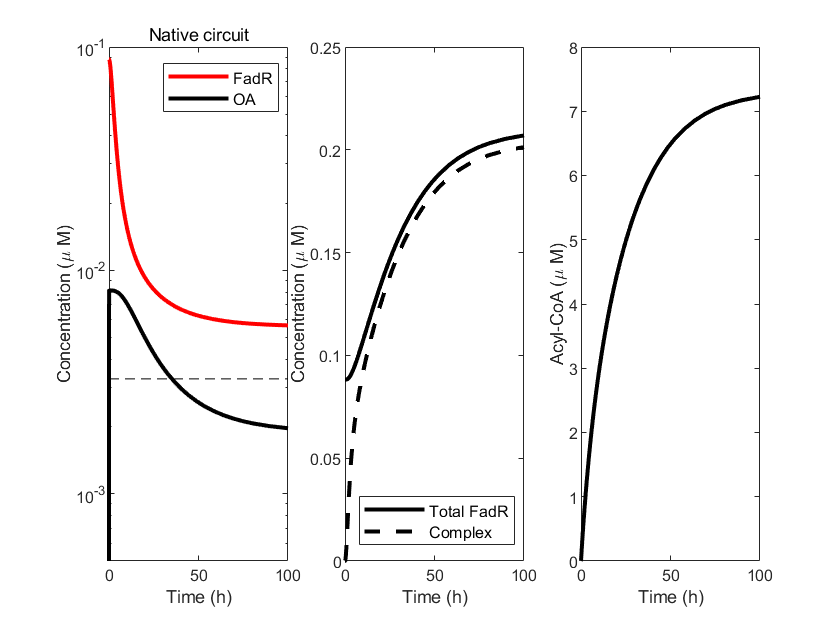
\includegraphics[width=0.75\linewidth]{figures/NAR_fig.png}
	\caption{Model Simulation of native circuit}
	\label{fig:NAR_fig}
\end{figure}

\begin{figure}[h]
	\centering
	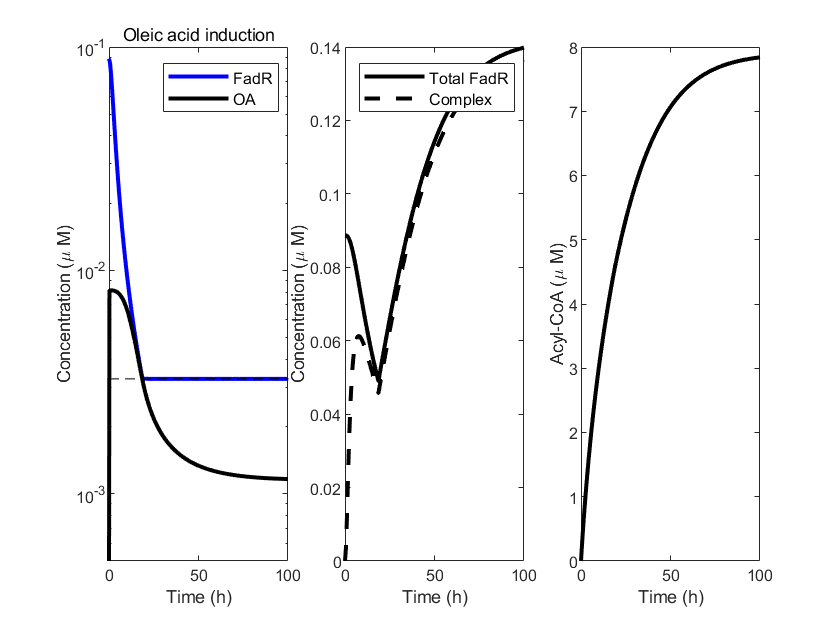
\includegraphics[width=0.75\linewidth]{figures/PAR_fig.png}
	\caption{Model Simulation of oleic acid inducer system}
	\label{fig:PAR_fig}
\end{figure}

From the plots, it is evident that, compared to the native circuit in Figure \ref{fig:NAR_fig}, the introduction of the oleic acid inducer in Figure \ref{fig:PAR_fig} accelerates the decomposition of OA into acyl-CoA(A) and its binding process with FadR, allowing the FadR concentration to decrease more rapidly to the threshold where the $P_{\mathrm{fadB}}$ in the oleic acid inducer is normally initiated. On the other hand, maintaining the FadR concentration at the threshold position for an extended period ensures the continuous activation of the oleic acid inducer, allowing the gene downstream of the artificially added FadO to be continuously expressed. This proves the effectiveness of the oleic acid inducer as a biological switch.

\subsection{Model expansion with additional FadO operators}

By modifying a segment of the FadO operator sequence in the promoter  region, we can alter the oleic acid concentration threshold required to  activate the promoter. Specifically, increasing the FadO operators  raises the threshold of oleic acid needed for acyl-CoA to dissociate  from FadR, allowing the PfadBPfadB promoter to initiate transcription normally. This mechanism sets a  higher bar for oleic acid inducer activation. With this approach,  through quantitative experimentation and mathematical modeling, we can  determine the appropriate induction initiation threshold range, which  aligns with the oleic acid content defined in high-fat diets for various individual physiologies. Consequently, this allows us to design  cholesterol-degrading bacterial strains based on the oleic acid inducer  principle, tailored to fit the gut nutritional environment of different  individuals.

\begin{figure}[h]
	\centering
	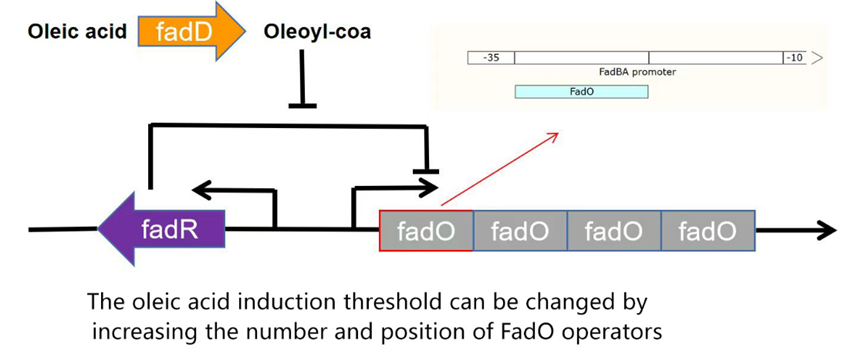
\includegraphics[width=0.75\linewidth]{figures/fado.png}
	\caption{The principle of model with additional FadO operators}
	\label{fig:fado}
\end{figure}

Similarly, we conducted model simulations to verify the feasibility of  the aforementioned operation. Specifically, we utilized an alternative  approach, adjusting the affinity of FadR to inhibit Ep synthesis within our system, to emulate the effects of modifying the FadO operators. A  higher affinity mimics the impact of having additional FadO operators,  necessitating a higher oleic acid concentration to activate the  promoter, and vice versa.


%\begin{figure}[h]
%	\centering
%	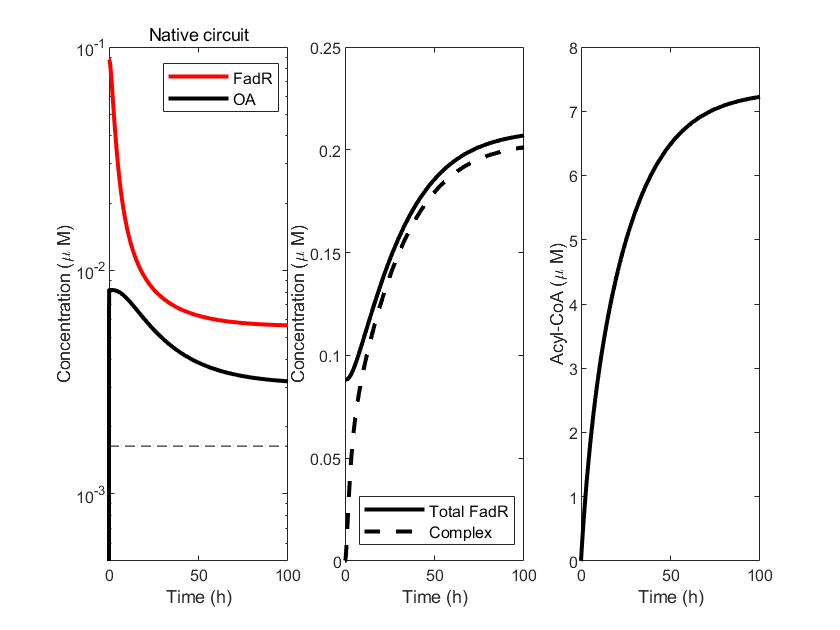
\includegraphics[width=0.8\linewidth]{figures/NAR_fig_fado.png}
%	\caption{Model Simulation of native circuit with additional FadO operators}
%	\label{fig:NAR_fig_fado}
%\end{figure}

\begin{figure}[h]
	\centering
	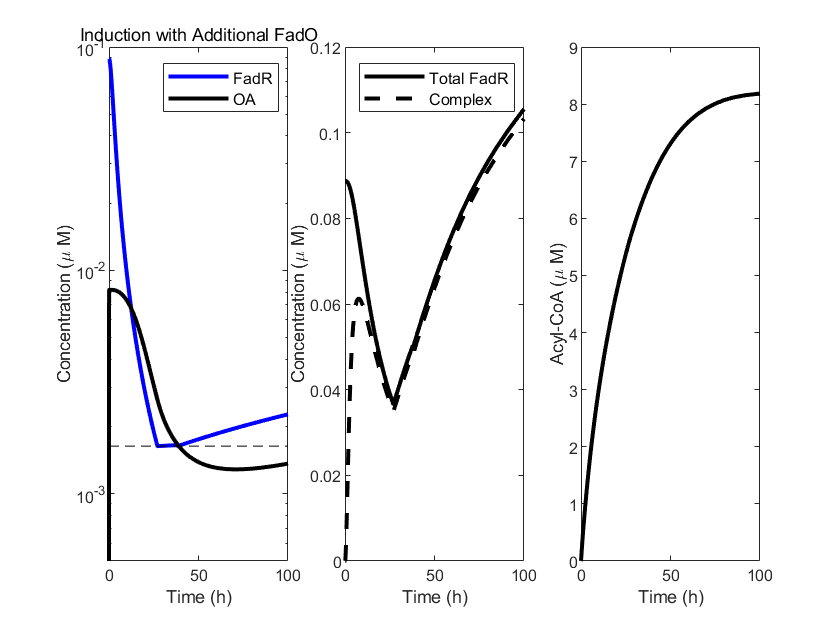
\includegraphics[width=0.75\linewidth]{figures/PAR_fig_fado.png}
	\caption{Model Simulation of oleic acid inducer system with additional FadO operators}
	\label{fig:PAR_fig_fado}
\end{figure}

In the additional FadO model simulation Figure \ref{fig:PAR_fig_fado}, we can observe that compared to the original oleic acid inducer, the new version with the added FadO not only slowed down the decomposition of OA but also shortened the time FadR remains at the activation threshold of the oleic acid inducer. Additionally, the activation threshold corresponding to FadR for the oleic acid inducer is lower. Given that the acyl-CoA (A) produced by the decomposition of oleic acid reacts with FadR and detaches from the FadO promoter p-fadB, this suggests that the inclusion of the FadO operator makes the oleic acid inducer harder to activate, consistent with our theoretical predictions. This validates that by introducing the FadO operator, we can precisely control the reaction threshold of the oleic acid inducer, making it adaptable to various scenarios.


\subsection{Parameter estimation by measuring the fluorescence intensity}

In the wet lab experiment, we introduced a fluorescent protein gene  downstream of the oleic acid inducer operator fadO. When FadR binds to  the operator fadO, it triggers the activation of the oleic acid inducer, leading to the expression of the fluorescent protein gene. Using this  data, we can correlate the changes in the variables simulated in our  original model with default parameters [1,2] to our actual experimental  data. This allows us to better interpret the experimental data and  provide guidance for subsequent experiments.

We tested the raw fluorescence intensity and OD600 (optical density at 600 nm) under three oleic acid concentrations: 5\%, 10\%, and 15\%, in both aerobic and anaerobic conditions. For each type, we conducted tests on six sets of data. Subsequently, we organized and preprocessed the respective experimental data to assist in subsequent parameter estimation. The data preprocessing steps include outlier handling and imputation and calculating the absolute fluorescence intensity. In each part, we adopted reliable strategies. The specific data and processing flow can be referred to in Appendix A.

First, we conducted a model simulation using default parameters to capture the characteristics of the system. To remain consistent with our experimental environment, instead of introducing oleic acid midway during this simulation, we quantitatively computed it by providing an initial oleic acid concentration. The results of the model simulation are shown in Figure 6. As observed, with the onset of the system operation, the concentration of oleic acid rapidly declines. The reaction results in the production of acyl-CoA (A), which combines with FadR, causing a swift decrease in the system's FadR concentration to a threshold, triggering the FadO switch. Correspondingly, the concentrations of variables like Total FadR, sequestered complex (C), and acyl-CoA also rise rapidly. Once the oleic acid reaction completes, FadR gradually regrows above the threshold, shutting off the FadO switch, marking the end of this activation phase of the oleic acid inducer. Throughout this process, we observe the fluorescence protein intensity gradually increasing to a stable value. Since this gene is downstream of the fadO operator, it can simulate the overall intensity of the fadO switch activation, paving the way for our subsequent quantitative calculations and parameter estimation.

\begin{figure}[h]
	\centering
	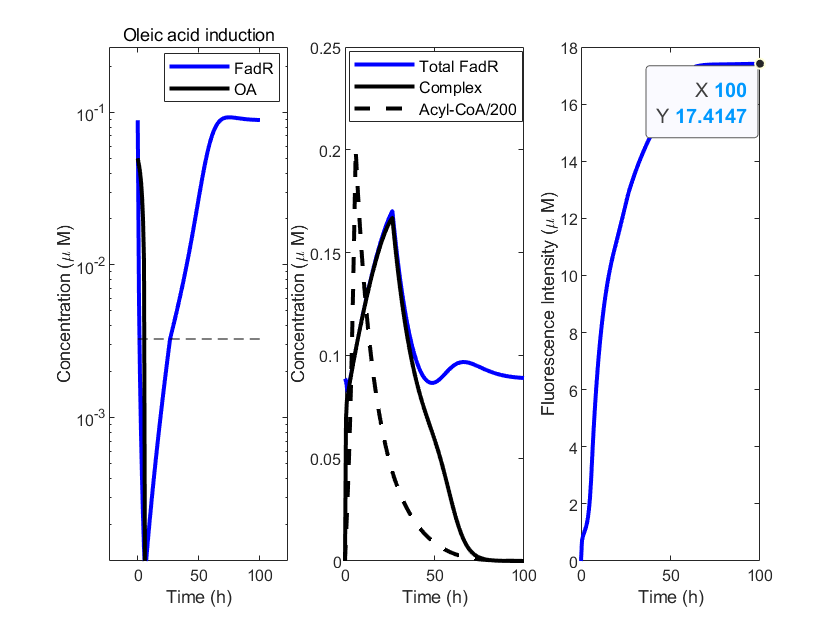
\includegraphics[width=0.75\linewidth]{figures/para_est_0mark.png}
	\caption{A visualization of fluorescence intensity F in the model}
	\label{fig:para_est_0}
\end{figure}

For the fluorescence intensity data, we roughly calculated the mean corrected absolute fluorescence intensity according to the following formulae. Below, we will briefly refer to it as Experiment(Exp) F to distinguish it from the fluorescence intensity F simulated in the model.

\begin{equation}
	\begin{gathered}
		A F I=\frac{R F I}{O D 600} \\
		\text { Corrected } A F I_{n \%}=A F I_{n \%}-E m p t y
	\end{gathered}
\end{equation}



Next, we embark on the model simulation section. To align with our  experimental setup, we did not introduce oleic acid midway during this  simulation. Instead, we conducted quantitative computations based on the provision of initial oleic acid concentrations. We simulated how each  variable in the model changes over time under three initial oleic acid  concentrations: 5\%, 10\%, and 15\%. Specifically, the first subplot  compares the expected fluorescence protein intensity under these three  initial oleic acid concentrations. The x-axis for the second and third  subplots represents the fluorescence protein intensity as simulated by  the model, while the y-axis shows the actual experimentally detected  fluorescence protein intensity. We employed linear regression to derive  reasonable model parameters, ensuring that the model can reflect the  outcomes of real data.
\begin{equation}
\text{Exp} \ F_{n\%}  = A \cdot AFI_{n\%} + B
\end{equation}


\begin{figure}[h]
	\centering
	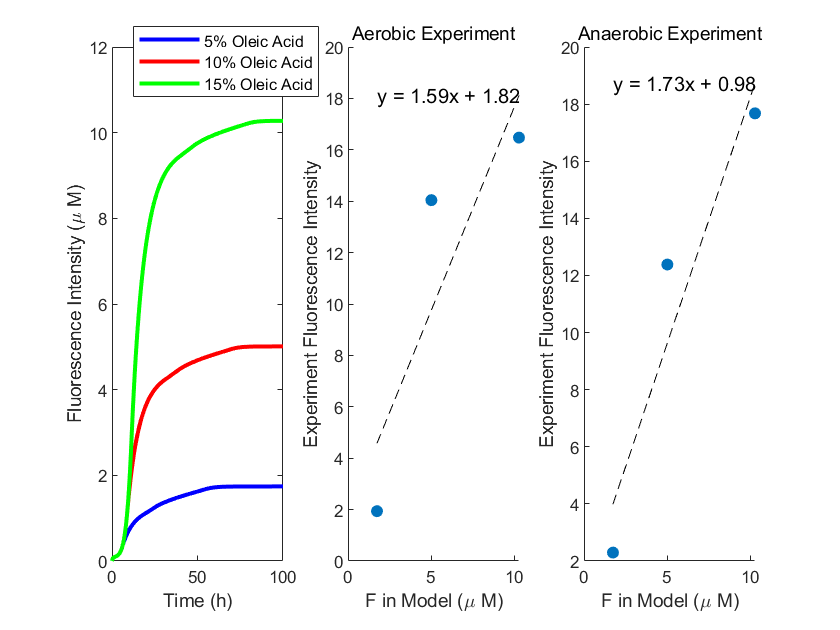
\includegraphics[width=0.75\linewidth]{figures/para_fit_fig.png}
	\caption{Parameter estimation by measuring the fluorescence intensity and fitting}
	\label{fig:parafit}
\end{figure}

From the figure, we can observe that higher oleic acid concentrations  lead to longer activation times for the oleic acid inducer. Taking into  account the initial degradation losses, the expression level of  fluorescent protein should increase faster than linearly with the growth of the initial oleic acid concentration. As for the fluorescence  intensity simulated by the model compared to the actual experimental  detection, we can see that the two are essentially in alignment, demonstrating the success of our experiment.

\section{Model Analysis}

\subsection{Model Stability}
To describe the behavior of our oleic acid inducer control system, we  examined the dose-response, that is, the system's steady state achieved  at different oleic acid concentrations. Here, we detailed how to  calculate the steady state and its stability for a given inducer  concentration. Here, in order to simulate the steady-state calculation of the entire system, we added a linear decay term $k$ for the fluorescence intensity $F$, which modifies the original equation to:
\begin{equation}
	\frac{d F}{d t}=r_{\mathrm{f}}-k
\end{equation}

$$
\text { Let } \frac{d F}{d t}=0, \quad \text {then }\quad r_{\text {f }}=k=k_{\mathrm{f}} A^2 R-k_{\mathrm{r}} C
$$

Also, let $$\frac{d E g}{d t}=0, \quad \text {then }  r_{\mathrm{x}, E_{\mathrm{g}}}=\lambda(E_g) E_g, \quad \lambda(E_ g)=E_g \lambda_{\text {min }}+\lambda_{\text {max }}-\lambda_{\text {min }}$$ 

Thus,  $$\frac{a_g \mathrm{K_g} R}{1+\mathrm{K_g} R} =E_g^2 \lambda_{\text {min }}+\left(\lambda_{\text {max }}-\lambda_{\text {min }}\right) E_g$$

From which we get: 
\begin{equation}
	E_g=\frac{-\lambda _\text {min}+\sqrt{\lambda_{\text {min }}^2+\frac{\lambda_{max}-\lambda_{\min }}{1+k_g R^2}} a_g k_g R }{2\left(\lambda_{\max }-\lambda_{\min }\right)}
\end{equation}

Letting (1), (2), (3), and (4) equal 0, when $r_{\mathrm{seq}}=k$ , we obtain:

\begin{equation}
	\left\{\begin{array}{l}
		R=\frac{r_{\mathrm{x}, \mathrm{R}}-k}{\lambda\left(E_g\right)} \\
		D=\frac{r_{\mathrm{x}, \mathrm{D}}}{\lambda (E_g)}=\frac{b_D+\frac{a D}{1+\frac{K_0^2}{\lambda (E_g)^2}\left(b_R-k+P_R(R)\right)^2}}{\lambda (E_g)} \\
		A=\frac{r_D-r_B-2 k}{\lambda (E_g)} \\
		C=\frac{K}{\lambda (E_g)}
	\end{array}\right.
\end{equation}

Based on the analysis, we only need to solve for $\lambda\left(E_g\right)$ to determine the other coefficients. And since $\lambda\left(E_g\right)$ is related to $R$, by solving for $R$, we can derive the other quantities.
Using the relation $R=\frac{r_{x, R}-k}{\lambda E_g}$ and substituting in $r_{x, R}=b_R+P_R(R)$, we get:
$$
\frac{-\lambda_{min }^2+\lambda_{min} \sqrt{\lambda_{min }{ }^2+\frac{4 a_g k_g R}{1+4 k_ g R}(\lambda_{max} -\lambda_{min} )}}{2\left(\lambda_{\max }-\lambda_{\min }\right)}+\lambda_{\max }-\lambda_{\min } -\frac{a_R}{1+k_R}=b_R-k
$$
After a series of simplifications, the final equation becomes a cubic equation in terms of $s$, where $s=t+c=\frac{a_R}{1+K_R R}+\left(b_2+\lambda_{\min }-\lambda_{\max }-k\right)$. Solving this gives the analytical solutions for $R=\frac{a_R-t}{t k_R}$ and $\lambda\left(E_g\right)$.

Through the above analysis and derivation, we provide analytical solutions for the steady states of different components in this oleic acid inducer system, offering a valuable starting point for further research and experiments.

\subsection{Model Sensitivity}
In this section, we conducted a global and local sensitivity analysis of the dose-response to parameter variations in the oleic acid inducer system.

For the global sensitivity analysis, we employed the eFAST [6] method to visualize the average and standard deviation (error bars) of the first-order sensitivity indices, as well as their values found in 100 parameter sets (dots). eFAST was implemented in MATLAB R2022a and explored values of parameters $b_R; a_R; K_R; b_D; a_D; K_D;S_T$ ranging from 10\% to 500\% of their default parameters as mentioned in [1,2]. 
\begin{figure}[h]
	\centering
	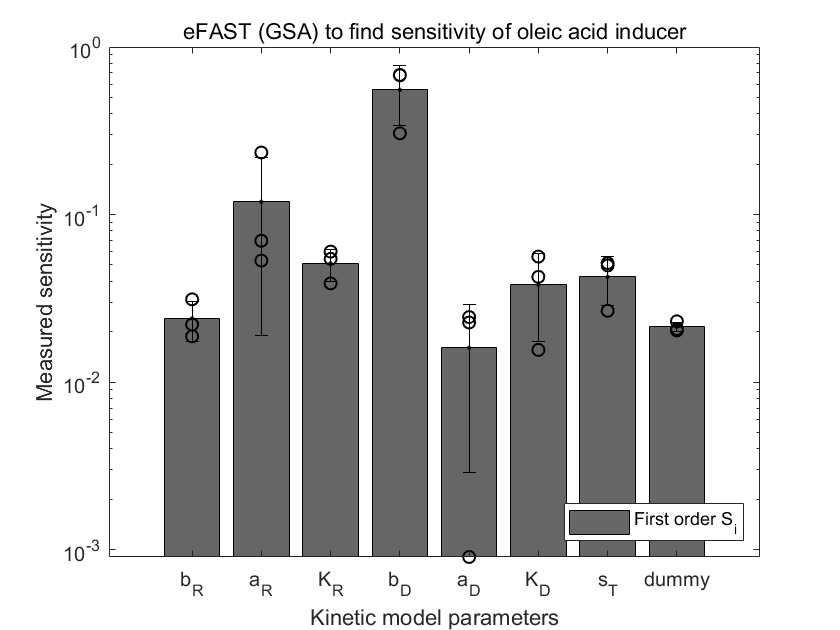
\includegraphics[width=0.75\linewidth]{figures/GSA_sen.png}
	\caption{Plots of average and standard deviation (error bars) of first-order sensitivity indices}
	\label{fig:GSA_sen}
\end{figure}

For the local sensitivity analysis, we constructed plots illustrating the dose-response changes when altering one parameter at a time [1]. Nine log-spaced values of several key parameters were sampled, ranging from 10\% to the nominal value presented in Supplementary Table 2 by 1000\%. The blue curve represents the nominal value.
\begin{figure}[h]
	\centering
	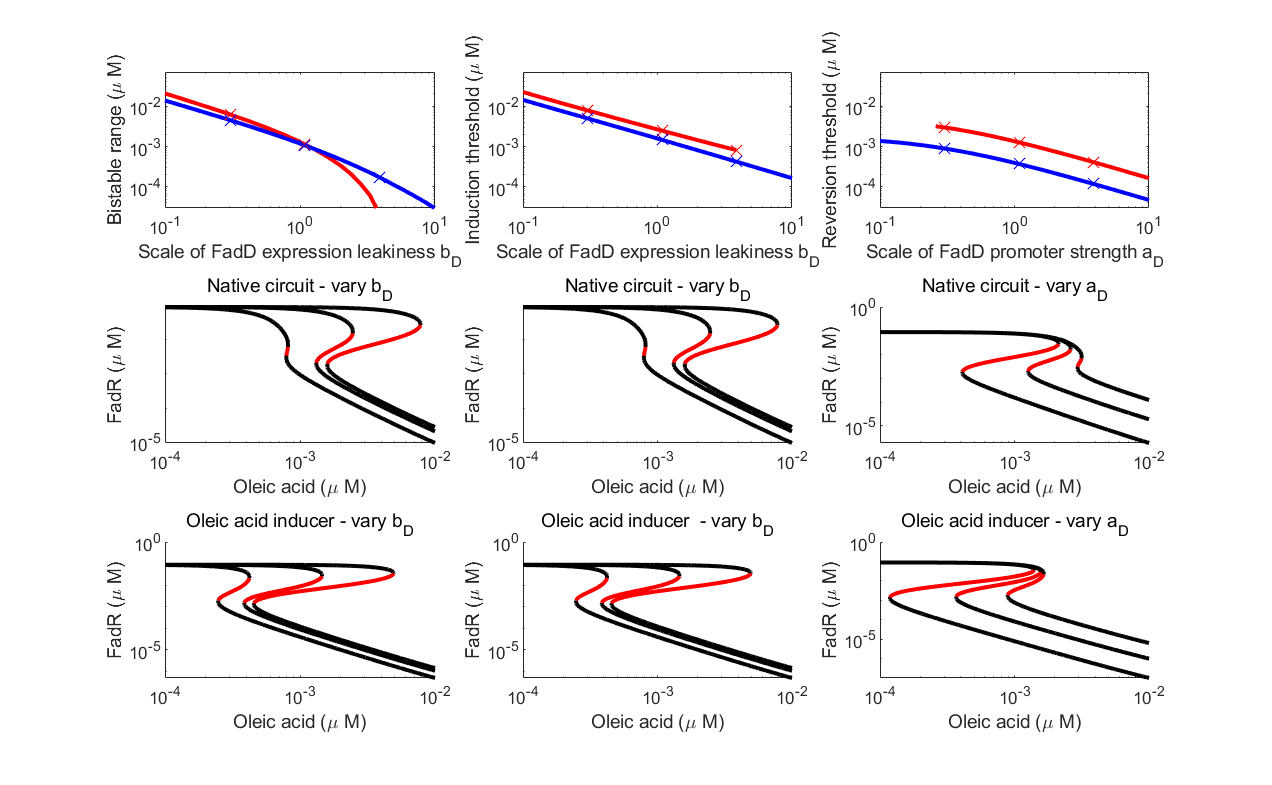
\includegraphics[width=0.85\linewidth]{figures/dr_sen_small.png}
	\caption{Plots of how dose-responsechanged for changes in one parameter at a time}
	\label{fig:dr_sen}
\end{figure}

\section*{References}

[1] Mannan, A.A., Bates, D.G. Designing an irreversible metabolic switch for scalable induction of microbial chemical production.                    *Nat Commun* **12**, 3419 (2021). 

[2] Hartline, C., Mannan, A., Liu, D., Zhang, F. \& Oyarz´un, D. Metabolite sequestration enables rapid recovery from fatty acid depletion in Escherichia coli. mBio (2020).

[3] Usui, Y. et al. Investigating the effects of perturbations to pgi and eno gene expression on central carbon metabolism in Escherichia coli using 13 C metabolic flux analysis. Microbial Cell Factories 11, 1–5 (2012).

[4] Mannan, A. A., Liu, D., Zhang, F. \& Oyarz´un, D. A. Fundamental design principles for transcription-factor-based metabo-lite biosensors. ACS Synthetic Biology 6, 1851–1859 (2017).

[5] Janßen, H. J. \& Steinb¨uchel, A. Fatty acid synthesis in Escherichia coli and its applications towards the production of fatty acid based biofuels. Biotechnology for biofuels 7, 7 (2014).

[6] Marino, S., Hogue, I. B., Ray, C. J. \& Kirschner, D. E. A methodology for performing global uncertainty and sensitivity analysis in systems biology. Journal of Theoretical Biology 254, 178–196 (2008).

[7] Bertram, R. \& Hillen, W. The application of Tet repressor in prokaryotic gene regulation and expression. Microbial Biotechnology 1, 2–16 (2008).

[8] Rohatgi, A. WebPlotDigitizer (2020). URL https://automeris.io/WebPlotDigitizer.

[9] Kamionka, A., Bogdanska-Urbaniak, J., Scholz, O. \& Hillen, W. Two mutations in the tetracycline repressor change the inducer anhydrotetracycline to a corepressor. Nucleic Acids Research 32, 842–847 (2004).

[10] Gardner, T. S., Cantor, C. R. \& Collins, J. J. Construction of a genetic toggle switch in Escherichia coli. Nature 403,339–342 (2000).

[11] Xu, J. \& Matthews, K. S. Flexibility in the Inducer Binding Region is Crucial for Allostery in the Escherichia coli Lactose Repressor. Biochemistry 48, 4988–4998.


\end{document}